\section{Auswertung}
\label{sec:auswertung}
%
Die in der Auswertung verwendeten Mittelwerte mehrfach gemessener Größen sind
gemäß der Gleichung
%
\begin{equation}
    \bar{x}=\frac{1}{n}\sum_{i=1}^n x_i
    \label{eq:mittelwert}
\end{equation}
%
bestimmt. Die Standardabweichung des Mittelwertes ergibt sich dabei zu
%
\begin{equation}
    \mathup{\Delta}\bar{x}=\sqrt{\frac{1}{n(n-1)}\sum_{i=1}^n\left(x_i-\bar{x}\right)^2}.
    \label{eq:standardabweichung}
\end{equation}
%
Resultiert eine Größe über eine Gleichung aus zwei anderen fehlerbehafteten
Größen, so berechnet sich der Gesamtfehler nach der Gaußschen
Fehlerfortpflanzung zu
%
\begin{equation}
    \mathup{\Delta}f(x_1,x_2,...,x_n)=\sqrt{\left(\frac{\partial f}{\partial x_1}\mathup{\Delta}x_1\right)^2+\left(\frac{\partial f}{\partial x_2}\mathup{\Delta}x_2\right)^2+ \dotsb +\left(\frac{\partial f}{\partial x_n}\mathup{\Delta}x_n\right)^2}.
    \label{eq:fehlerfortpflanzung}
\end{equation}
%
Alle in der Auswertung angegebenen Größen sind stets auf die erste signifikante
Stelle des Fehlers gerundet. Setzt sich eine Größe über mehrere Schritte aus
anderen Größen zusammen, so wird erst am Ende gerundet, um Fehler zu vermeiden.
Zur Auswertung wird die Programmiersprache \texttt{python (Version 3.4.1)} mit
den Bibliothekserweiterungen \texttt{numpy}~\cite{numpy},
\texttt{scipy}~\cite{scipy} und \texttt{matplotlib}~\cite{matplotlib} zur
Erstellung der Grafiken und linearen Regressionen verwendet.

In der folgenden Auswertung werden die Fehler von Größen immer durch
ein~$\Updelta$ kenntlich gemacht. Für die benötigten Zeit-, Temperatur- und
Energiedifferenzen wird ein~$\delta$ verwendet.
%
\subsection{Bestimmung der Molwärme von Kupfer}

Die molare Wärmekapazität~$C$ eines Stoffes berechnet sich im Experiment aus
dem Differenzenquotienten
%
\begin{equation}
  C=\frac{\delta E}{\delta T},
\end{equation}
%
der abgeleitet ist aus der thermodynamischen Relation in
Gleichung~\eqref{eq:CV}. Die der Kupferprobe durch die Heizwicklung zugeführte
elektrische Energie~$\delta E$ berechnet sich dabei gemäß
%
\begin{equation}
  \delta E = UI\delta t
\end{equation}
%
aus den Messdaten für die Spannung~$U$ und den Strom~$I$ der Heizwicklung. Das
gemessene Zeitintervall beträgt stets~$\delta t=\SI{300(1)}{\second}$. Dabei
resultiert der angegebene Fehler aus der Ablesegenauigkeit des verwendeten
Zeitmessers. Die benötigte Temperaturdifferenz~$\delta T$ wird aus den
gemessenen Widerständen~$R$ bestimmmt. Die zugehörige Umrechnungsformel lautet
%
\begin{gather}
  T=\SI{0.00134}{\kelvin\per\ohm\squared}R^2+\SI{2.296}{\kelvin\per\ohm}R-\SI{30.13}{\kelvin} \\
  \shortintertext{mit dem Fehler}
  \Updelta T=\left(\SI{0.00268}{\kelvin\per\ohm}+\SI{2.296}{\kelvin}\right)\SI{}{\per\ohm}\Updelta R
\end{gather}
%
und ist~\cite{V47} entnommen. Es soll die Wärmekapazität bei konstantem
Volumen~$C_{\mathrm{V}}$ berechnet werden. Da temperaturabhängige Messungen bei
konstantem Volumen an einem Festkörper jedoch schwer durchzuführen sind, wird
die Messung ersatzweise bei konstantem Druck durchgeführt.
Die auf die Stoffmenge~$n=\sfrac{m}{M}$ bezogene molare Wärmekapazität bei
konstantem Druck~$C_{\mathrm{P}}$ ergibt sich, abgeleitet aus
Gleichung~\eqref{TODO}, zu
%
\begin{gather}
  C_{\mathrm{P}}=\frac{UI\delta t}{\delta T}\frac{M}{m} \\
  \intertext{mit dem Fehler}
  \Updelta C_{\mathrm{P}}=\frac{M}{m}\sqrt{\left(\frac{I\delta t}{\delta T}\Updelta U\right)^2+\left(\frac{U\delta t}{\delta T}\Updelta I\right)^2+\left(\frac{UI}{\delta T}\Updelta(\delta t)\right)^2+\left(\frac{UI\delta t}{(\delta T)^2}\Updelta(\delta T)\right)^2}.
\end{gather}
%
Hierbei ist~$M=\SI{63.546}{\gram\per\mol}$~\cite{mathematica} die molare Masse
von Kupfer und~$m=\SI{0.342}{\kilo\gram}$~\cite{V47} die Masse der Probe. Die
Umrechnung von~$C_{\mathrm{P}}$ in~$C_{\mathrm{V}}$ erfolgt mit Hilfe der
Gleichung
%
\begin{gather}
  C_{\mathrm{V}}=C_{\mathrm{P}}-9\alpha^2\kappa V_0T\label{eq:Cp2Cv} \\
  \intertext{und hat den Fehler}
  \Updelta C_{\mathrm{V}}=\sqrt{(\Updelta C_{\mathrm{P}})^2+(18\alpha\kappa V_0T\Updelta\alpha)^2+(9\alpha^2\kappa V_0\Updelta T)^2}.
\end{gather}
%
$\alpha$ ist der temperaturabhängige lineare Ausdehnungskoeffizient, für den in
Tabelle~\ref{tab:ausdehnungskoeffizient} einige Werte bei verschiedenen
Temperaturen angegeben sind. Das Kompressionsmodul~$\kappa$ von Kupfer beträgt
nach~\cite{mathematica}
%
\begin{equation}
  \kappa=\SI{140}{\giga\newton\per\metre\squared}.
\end{equation}
%
Das molare Volumen~$V_0$ der verwendeten Probe berechnet sich mit Hilfe der
Avogadro-Konstanten~$N_{\mathrm{A}}=\SI{6.022e23}{\per\mol}$ aus der
Dichte~$\rho=\SI{8.960}{\gram\per\centi\metre\cubed}$~\cite{mathematica} und der
molaren Masse~$M$ zu
%
\begin{equation}
  V_0=\frac{M}{\rho}=\SI{7.092e-6}{\metre\cubed\per\mol}.
\end{equation}

\begin{table}[htb]
    \centering
    \caption{Linearer Ausdehnungskoeffizient~$\alpha$ von Kupfer in Abhängigkeit
    der Temperatur~$T$ \cite{V47}.}
    \begin{tabular}{S[table-format = 3.0]
                    S[table-format = 2.2] |
                    S[table-format = 3.0]
                    S[table-format = 2.2] }
        \toprule
        {$T$ in \si{\kelvin}} & {$\alpha\cdot 10^{-6}$ in \si{\per\kelvin}} & {$T$ in \si{\kelvin}} & {$\alpha\cdot 10^{-6}$ in \si{\per\kelvin}} \\
        \midrule
         70 &  7.00 & 190 & 14.75 \\
         80 &  8.50 & 200 & 14.95 \\
         90 &  9.75 & 210 & 15.20 \\
        100 & 10.70 & 220 & 15.40 \\
        110 & 11.50 & 230 & 15.60 \\
        120 & 12.10 & 240 & 15.75 \\
        130 & 12.65 & 250 & 15.90 \\
        140 & 13.15 & 260 & 16.10 \\
        150 & 13.60 & 270 & 16.25 \\
        160 & 13.90 & 280 & 16.35 \\
        170 & 14.25 & 290 & 16.50 \\
        180 & 14.50 & 300 & 16.65 \\
        \bottomrule
    \end{tabular}
    \label{tab:ausdehnungskoeffizient}
\end{table}

Der Ausdehnungskoeffizient von Festkörpern hat eine~$T^{-1}$-Abhängigkeit.
Der daraus resultierende lineare Fit der Form
%
\begin{gather}
  \alpha(T)=m\frac{1}{T}+b \\
  \shortintertext{mit dem Fehler}
  \Updelta\alpha(T,\Updelta T)=\sqrt{\left(\frac{1}{T}\Updelta m\right)^2+\left(\frac{m}{T^2}\Updelta T\right)^2+(\Updelta b)^2}
\end{gather}
%
ist zusammen mit den gegebenen Stützstellen in Abbildung~\ref{fig:plot_alpha}
aufgetragen. Der Fit liefert für die Parameter~$m$ und~$b$ die Werte
%
\begin{gather}
  m = \SI{-873(4)e-6}{} \\           % -0.000872928077602 +- 4.12768256344e-06
  \shortintertext{und}
  b = \SI{19.41(3)e-6}{\per\kelvin}. %  1.94110943588e-05 +- 2.92795520852e-08
\end{gather}
%
Die weiteren für Gleichung~\eqref{eq:Cp2Cv} benötigten Parameter werden der
Literatur entnommen.
%
\begin{figure}[htb]
    \centering
    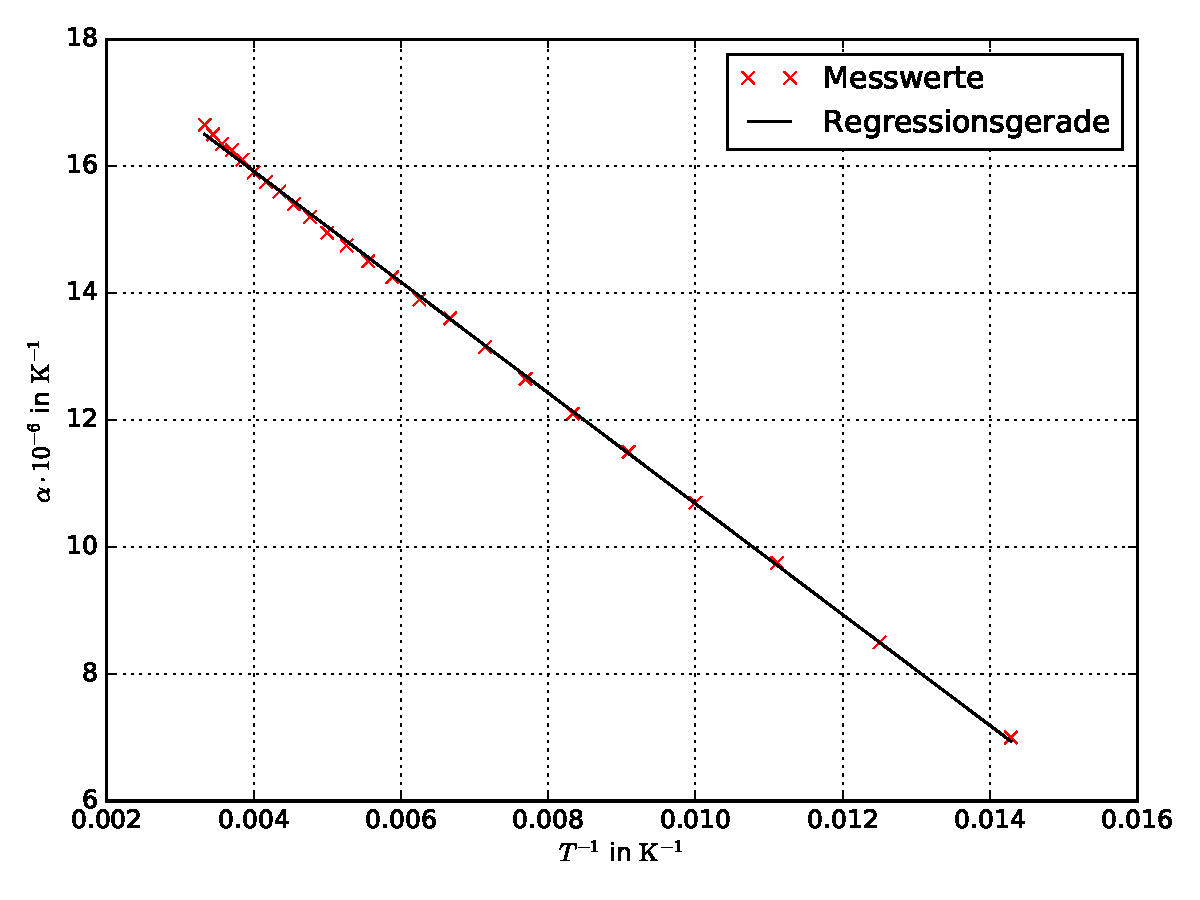
\includegraphics[width=\textwidth]{content/plot_alpha.pdf}
    \caption{Linearer Ausdehnungskoeffizient~$\alpha$ von Kupfer aufgetragen
    gegen die inverse Temperatur.}
    \label{fig:plot_alpha}
\end{figure}
%
Tabelle~\ref{tab:Molwaerme} zeigt zusammenfassend alle Messdaten
sowie die zugehörigen berechneten Größen. In Abbildung~\ref{fig:plot_Cv} sind
die berechneten Werte für~$C_{\mathrm{P}}$ und~$C_{\mathrm{V}}$ samt
Fehlerbalken gegen die Temperatur aufgetragen dargestellt.

\begin{figure}[htb]
    \centering
    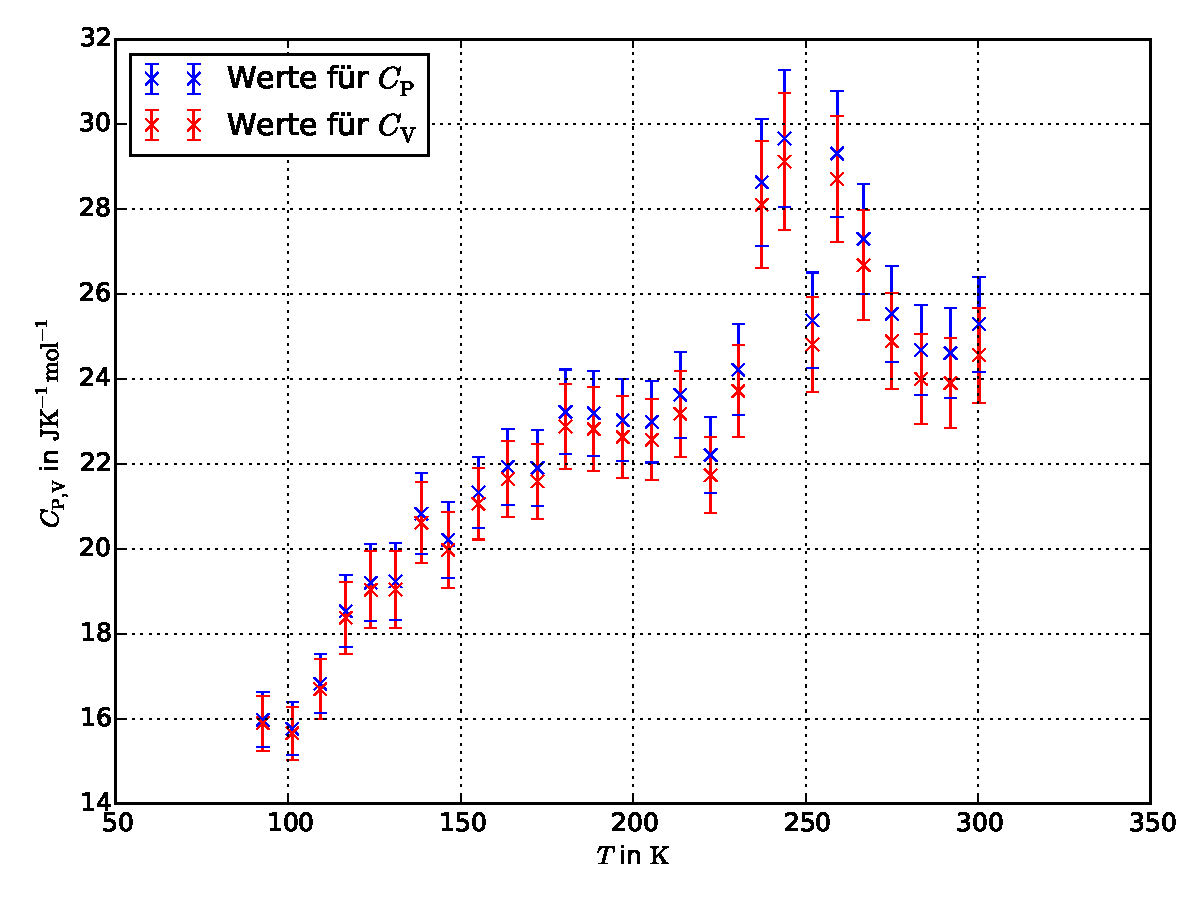
\includegraphics[width=\textwidth]{content/plot_Cv.pdf}
    \caption{Berechnete Werte für~$C_{\mathrm{P}}$ und~$C_{\mathrm{V}}$
    aufgetragen gegen die Temperatur. Im Bereich zwischen~\SI{100}{\kelvin}
    und~\SI{170}{\kelvin} ist der Verlauf annähernd linear.}
    \label{fig:plot_Cv}
\end{figure}

\subsection{Bestimmung der Debye-Temperatur}
%
Ziel ist es nun die Debye-Temperatur~$\theta_{\mathrm{D}}$ der Kupferprobe zu
bestimmen. Nach Gleichung~\eqref{eq:debyetemperatur} gilt
%
\begin{gather}
  \theta_{\mathrm{D}}=T\sqrt[3]{\frac{9R}{C_{\mathrm{V}}}f\left(\frac{\theta_{\mathrm{D}}}{T}\right)}
  \shortintertext{mit dem Fehler} \\
  \Updelta\theta_{\mathrm{D}}=\sqrt{\left(\sqrt[3]{\frac{9R}{C_{\mathrm{V}}}f\left(\frac{\theta_{\mathrm{D}}}{T}\right)}\Updelta T\right)^2+\left(T\sqrt[3]{\frac{R}{9C_{\mathrm{V}}^4}f\left(\frac{\theta_{\mathrm{D}}}{T}\right)}\Updelta C_{\mathrm{V}}\right)^2}.
\end{gather}
%
Die hierfür benötigten Werte der
Debye-Funktion~$f\left(\frac{\theta_{\mathrm{D}}}{T}\right)$ können in
Tabelle~1 in~\cite{V47} abgelesen werden. $R=\SI{8.314}{\joule\per\mol\kelvin}$
ist die allgemeine Gaskonstante. Es werden nur die Werte~$C_{\mathrm{V}}$
betrachtet, die zu einer Temperatur~$T<\SI{170}{\kelvin}$ bestimmt wurden. Die
errechneten Werte für~$\theta_{\mathrm{D}}$ sind in
Tabelle~\ref{tab:debyetemperatur} zusammengefasst. Als Mittelwert ergibt sich
%
\begin{equation}
  \theta_{\mathrm{D},1}=\SI{269(5)}{\kelvin}. % 268.70231530285855 +- 4.6632930701167385
\end{equation}
%
\begin{table}[H]
    \centering
    \caption{Gemessene und berechnete physikalische Größen zur Bestimmung der
    Debye-Temperatur~$\theta_{\mathrm{D}}$ einer Kupferprobe.}
    \begin{tabular}{S[table-format=3.1,separate-uncertainty,table-figures-uncertainty=1]
                    S[table-format=2.1,separate-uncertainty,table-figures-uncertainty=1]
                    S
                    S[table-format=3.0,separate-uncertainty,table-figures-uncertainty=1]}
        \toprule
        {$T$ in \si{\kelvin}} & {$C_{\mathrm{V}}$ in \si{\joule\per\mol\per\kelvin}} & {$f\left(\frac{\theta_{\mathrm{D}}}{T}\right)$} & {$\theta_{\mathrm{D}}$ in \si{\per\kelvin}} \\
        \midrule
         92.6(2) & 15.9(6) & 3.2 & 229(3) \\
        101.2(2) & 15.7(6) & 3.2 & 251(4) \\
        109.3(2) & 16.7(7) & 3.0 & 260(4) \\
        116.7(2) & 18.3(8) & 2.6 & 256(5) \\
        123.9(2) & 19.0(9) & 2.4 & 262(5) \\
        131.1(2) & 19.0(9) & 2.4 & 277(5) \\
        138.6(2) & 21(1)   & 2.0 & 268(5) \\
        146.3(2) & 20.0(9) & 2.2 & 296(6) \\
        155.1(2) & 21.0(8) & 1.9 & 293(5) \\
        163.6(2) & 21.6(9) & 1.7 & 295(5) \\
        \bottomrule
    \end{tabular}
    \label{tab:debyetemperatur}
\end{table}
%
Ein alternativer Ansatz ermöglicht die Berechnung der Debye-Temperatur aus
Forderung~\eqref{eq:konv}. Es ergibt sich
%
\begin{equation}
  \theta_{\mathrm{D},2}=\frac{\hbar}{k_{\mathrm{B}}}\sqrt[3]{\frac{18\pi^2N_A\rho}{M}\left(v_{\mathrm{long}}^{-3}+2v_{\mathrm{trans}}^{-3}\right)^{-1}}=\SI{332,5}{\kelvin},
\end{equation}
%
wobei~$v_{\mathrm{long}}=\SI{4.7}{\kilo\metre\per\second}$ und $v_{\mathrm{trans}}=\SI{2.26}{\kilo\metre\per\second}$ verwendet wurde.
Für die Debye-Frequenzen ergeben sich die Werte
%
\begin{align}
  \omega_{\mathrm{D},1}&=\frac{k_{\mathrm{B}}}{\hbar}\theta_{\mathrm{D},1}=\SI{35.2(6)}{\tera\hertz} \\
  \shortintertext{und}
  \omega_{\mathrm{D},2}&=\frac{k_{\mathrm{B}}}{\hbar}\theta_{\mathrm{D},2}=\SI{43.53}{\tera\hertz}.
\end{align}

\begin{landscape}
  \begin{table}[htb]
    \centering
    \caption{Gemessene und berechnete physikalische Größen zur Bestimmung der
    molaren Wärmekapazität einer Kupferprobe.}
    \begin{tabular}{S[table-format=2.1,separate-uncertainty,table-figures-uncertainty=1]
                    S[table-format=2.2,separate-uncertainty,table-figures-uncertainty=1]
                    S[table-format=3.1,separate-uncertainty,table-figures-uncertainty=1]
                    S[table-format=3.1,separate-uncertainty,table-figures-uncertainty=1]
                    S[table-format=1.3,separate-uncertainty,table-figures-uncertainty=1]
                    S[table-format=1.1,separate-uncertainty,table-figures-uncertainty=1]
                    S[table-format=2.1,separate-uncertainty,table-figures-uncertainty=1]
                    S[table-format=2.1,separate-uncertainty,table-figures-uncertainty=1]}
        \toprule
        {$R$ in \si{\ohm}} & {$U$ in \si{\volt}} & {$I$ in \si{\milli\ampere}} & {$T$ in \si{\kelvin}} & {$\alpha\cdot10^{-5}$ in \si{\per\kelvin}} & {$\delta T$ in \si{\kelvin}} & {$C_{\mathrm{P}}$ in \si{\joule\per\mol\per\kelvin}} & {$C_{\mathrm{V}}$ in \si{\joule\per\mol\per\kelvin}} \\
        \midrule
         23.3(1) &  0.00    &   0.0    &  84.4(2) & 0.906(6) & {-}    & {-}     & {-}     \\
         26.8(1) & 15.75(1) & 150.5(1) &  92.6(2) & 0.999(6) & 8.3(3) & 16.0(6) & 15.9(6) \\
         30.4(1) & 15.91(1) & 151.8(1) & 101.2(2) & 1.078(5) & 8.5(3) & 15.8(6) & 15.7(6) \\
         33.8(1) & 16.02(1) & 152.6(1) & 109.3(2) & 1.142(5) & 8.1(3) & 16.8(7) & 16.7(7) \\
         36.9(1) & 16.09(1) & 153.1(1) & 116.7(2) & 1.193(5) & 7.4(3) & 18.5(8) & 18.3(8) \\
         39.9(1) & 16.15(1) & 153.5(1) & 123.9(2) & 1.236(5) & 7.2(3) & 19.2(9) & 19.0(9) \\
         42.9(1) & 16.20(1) & 153.8(1) & 131.1(2) & 1.275(4) & 7.2(3) & 19.2(9) & 19.0(9) \\
         46.0(1) & 17.17(1) & 162.9(1) & 138.6(2) & 1.311(4) & 7.5(3) & 21(1)   & 21(1)   \\
         49.2(1) & 17.22(1) & 163.3(1) & 146.3(2) & 1.345(4) & 7.8(3) & 20.2(9) & 20.0(9) \\
         52.8(1) & 18.80(1) & 178.2(1) & 155.1(2) & 1.378(4) & 8.8(3) & 21.3(8) & 21.0(8) \\
         56.3(1) & 18.84(1) & 178.5(1) & 163.6(2) & 1.408(4) & 8.5(3) & 21.9(9) & 21.6(9) \\
         59.8(1) & 18.87(1) & 178.7(1) & 172.2(2) & 1.434(4) & 8.6(3) & 21.9(9) & 21.6(9) \\
         63.1(1) & 18.90(1) & 179.0(1) & 180.3(2) & 1.457(4) & 8.1(3) & 23(1)   & 23(1)   \\
         66.4(1) & 18.92(1) & 179.2(1) & 188.5(2) & 1.478(4) & 8.1(3) & 23(1)   & 23(1)   \\
         69.8(1) & 19.18(1) & 181.5(1) & 196.9(2) & 1.498(4) & 8.4(4) & 23(1)   & 23(1)   \\
         73.2(1) & 19.20(1) & 181.7(1) & 205.4(2) & 1.516(4) & 8.5(4) & 23(1)   & 23(1)   \\
         76.5(1) & 19.21(1) & 181.8(1) & 213.6(3) & 1.532(4) & 8.2(4) & 24(1)   & 23(1)   \\
         80.0(1) & 19.22(1) & 181.8(1) & 222.4(3) & 1.549(3) & 8.8(4) & 22.2(9) & 21.7(9) \\
         83.2(1) & 19.22(1) & 181.9(1) & 230.4(3) & 1.562(3) & 8.0(4) & 24(1)   & 24(1)   \\
         85.9(1) & 19.22(1) & 182.0(1) & 237.2(3) & 1.573(3) & 6.8(4) & 28(2)   & 28(2)   \\
         88.5(1) & 19.23(1) & 182.0(1) & 243.8(3) & 1.583(3) & 6.6(4) & 30(2)   & 29(2)   \\
         91.7(1) & 19.74(1) & 187.3(1) & 251.9(3) & 1.595(3) & 8.1(4) & 25(1)   & 25(1)   \\
         94.5(1) & 19.89(1) & 188.4(1) & 259.1(3) & 1.604(3) & 7.1(4) & 29(1)   & 28(1)   \\
         97.5(1) & 19.89(1) & 188.6(1) & 266.7(3) & 1.613(3) & 7.7(4) & 27(1)   & 27(1)   \\
        100.7(1) & 19.90(1) & 188.7(1) & 274.9(3) & 1.624(3) & 8.2(4) & 26(1)   & 25(1)   \\
        104.0(1) & 19.90(1) & 188.7(1) & 283.4(3) & 1.633(3) & 8.5(4) & 25(1)   & 24(1)   \\
        107.3(1) & 19.90(1) & 188.8(1) & 291.9(3) & 1.642(3) & 8.5(4) & 25(1)   & 24(1)   \\
        110.5(1) & 19.90(1) & 188.8(1) & 300.2(3) & 1.650(3) & 8.3(4) & 25(1)   & 25(1)   \\
        \bottomrule
    \end{tabular}
    \label{tab:Molwaerme}
  \end{table}
\end{landscape}
